\documentclass[11pt]{article}

\input{./preamble.tex}

%%
%% DOCUMENT START
%%

\begin{document}

\renewcommand*{\arraystretch}{1.5}

\pagestyle{fancyplain}
\lhead{}
\chead{}
\rhead{}
\lfoot{\hrule UQ: Homework 1}
\cfoot{\hrule \thepage}
\rfoot{\hrule Ryan Skinner}

\noindent
{\Large Homework 1}
\hfill
{\large Ryan Skinner}
\\[0.5ex]
{\large ASEN 6519: Uncertainty Quantification}
\hfill
{\large Due 2016/02/23}\\
\hrule
\vspace{6pt}

%%%%%%%%%%%%%%%%%%%%%%%%%%%%%%%%%%%%%%%%%%%%%%%%%
%%%%%%%%%%%%%%%%%%%%%%%%%%%%%%%%%%%%%%%%%%%%%%%%%
\section*{Problem 1} %%%%%%%%%%%%%%%%%%%%%%%%%%%%
%%%%%%%%%%%%%%%%%%%%%%%%%%%%%%%%%%%%%%%%%%%%%%%%%
%%%%%%%%%%%%%%%%%%%%%%%%%%%%%%%%%%%%%%%%%%%%%%%%%

Let random variable X follow the Chebyshev probability density function
\begin{equation}
f_X(x) = \pi^{-1} (1 - x^2)^{-1/2}, \qquad x \in (-1, +1).
\end{equation}
Use the inversion method to generate 10,000 samples of $X$. To verify the quality of the generated samples, compare the empirical density and distribution functions of $X$ (based on the generated samples) to the exact values. You may use MATLAB functions `ksdensity` and `ecdf` to compute the empirical density and distribution functions, respectively.

\begin{figure}[h]
\centering
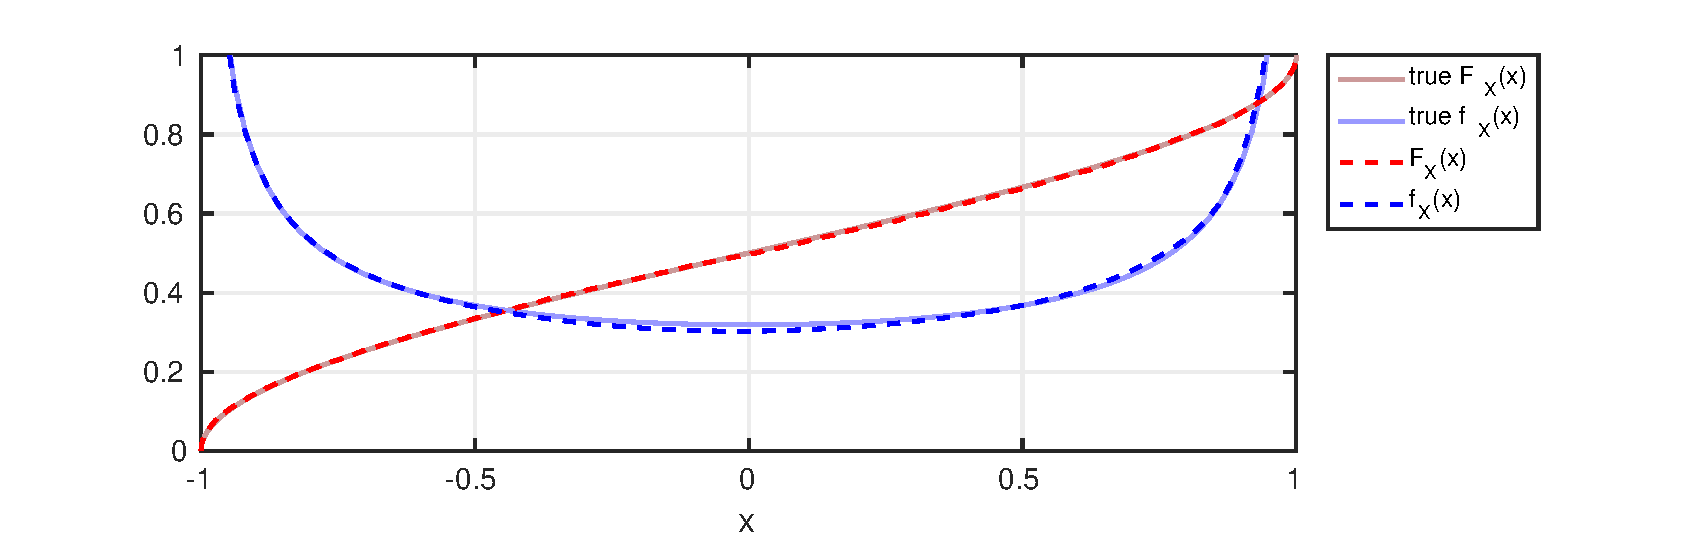
\includegraphics[width=\textwidth]{Prob1.eps}
\caption{Cumulative density function $F_X(x)$ and probability density function $f_X(x)$ based on analytical arguments and the inversion method using $N=10,\!000$ samples.}
\end{figure}

%%%%%%%%%%%%%%%%%%%%%%%%%%%%%%%%%%%%%%%%%%%%%%%%%
%%%%%%%%%%%%%%%%%%%%%%%%%%%%%%%%%%%%%%%%%%%%%%%%%
\section*{Problem 2} %%%%%%%%%%%%%%%%%%%%%%%%%%%%
%%%%%%%%%%%%%%%%%%%%%%%%%%%%%%%%%%%%%%%%%%%%%%%%%
%%%%%%%%%%%%%%%%%%%%%%%%%%%%%%%%%%%%%%%%%%%%%%%%%

$G(x, \omega)$ is a Gaussian random process defined on $(0, 1)$. The mean and covariance functions of the Gaussian process $G(x, \omega)$ are
\begin{equation}
\xpect{G(x)} = 1.0, \qquad x \in (0,1),
\end{equation}
and
\begin{equation}
C_{GG}(x_1,x_2) = \sigma^2 \exp \left( \frac{- | x_1-x_2 | }{\ell} \right), \qquad (x1,x2) \in (0,1) \times (0,1),
\end{equation}
respectively. We would like to compute the eigen-pairs of $C_{GG}(x_1,x_2)$ using the Galerkin approach with linear finite elements (or the Nystr\"om approach) and compare them with the exact values provided in the notes.

For $(\sigma, \ell)$ of $(2,2)$ and $(2,0.2)$, we compute the number of terms required in the KL expansion of $G(x,\omega)$ such that the mean-square error of truncation is roughly 10\%. Then, we verify the increasing the finite element resolution reduces error of the Galerkin estimated eigenvalues. Finally, we draw 100,000 samples of the random process, plot seven of them, and compute the mean and variance of all samples, comparing them to the given values.

\begin{figure}
\centering
\begin{subfigure}{0.49\textwidth}
\includegraphics[width=\textwidth]{Prob2a1.eps}
\includegraphics[width=\textwidth]{Prob2a2.eps}
\caption{$\ell=2$}
\end{subfigure}
\begin{subfigure}{0.49\textwidth}
\includegraphics[width=\textwidth]{Prob3a1.eps}
\includegraphics[width=\textwidth]{Prob3a2.eps}
\caption{$\ell=0.2$}
\end{subfigure}
\\[0.2cm]
\caption{1,000 analytical eigenvalues and normalized sum of the largest $b$ eigenvalues using $\sigma = 2$. Mean-square error of truncation $<10\%$ is first achieved with (a) $b=3$ and (b) $b=12$ terms in the KL expansion.}
\label{fig:analytical_eigs}
\end{figure}

\begin{figure}
\centering
\begin{subfigure}{0.49\textwidth}
\includegraphics[width=\textwidth]{Prob2b.eps}
\caption{$\ell=2$}
\end{subfigure}
\begin{subfigure}{0.49\textwidth}
\includegraphics[width=\textwidth]{Prob3b.eps}
\caption{$\ell=0.2$}
\end{subfigure}
\\[0.2cm]
\caption{Increasing the number of finite elements ($N_\text{el}=[N-1]^2$) increases accuracy of eigenvalues. For both plots, $\sigma=2$.}
\label{fig:error_reduction}
\end{figure}

\begin{figure}
\centering
\begin{subfigure}{0.49\textwidth}
\includegraphics[width=\textwidth,trim={0 1cm 0 0}]{Prob2cd.eps}
\caption{$\ell=2$}
\end{subfigure}
\begin{subfigure}{0.49\textwidth}
\includegraphics[width=\textwidth,trim={0 1cm 0 0}]{Prob3cd.eps}
\caption{$\ell=0.2$}
\end{subfigure}
\\[0.2cm]
\caption{From top to bottom: seven realizations of the random process $G(x,\omega)$, sample mean $\xpect{G(x)}$, and sample variance $\var(G(x))$, using 100,000 samples. For both plots, $\sigma=2$ and the KL expansion is used with $b(\ell)$ terms.}
\label{fig:realizations}
\end{figure}

In \figref{fig:analytical_eigs}, we see that a longer correlation length $\ell$ is associated with a more rapid decay in eigenvalues. More eigenfunctions are necessary to capture the higher-frequency dynamics of systems with small correlation length, and thus their eigenvalues decay less rapidly.

In \figref{fig:error_reduction}, as expected, increasing the number of finite elements decreases the relative error of our approximated eigenvalues. The larger the magnitude of $\lambda_i$, the lower its relative error. Smaller correlation length $\ell$ corresponds to reduced eigenvalue accuracy for a given number of finite elements.

In \figref{fig:realizations}, we see the high-frequency behavior implied by smaller $\ell$ manifest in the seven individual realizations. For both $\ell=2$ and $\ell=0.2$, the sample mean matches the true mean very well; this is a direct consequence of reducing the mean square error to $<10\%$. The variance is less accurate, however, because it is a higher-order statistic. Larger $\ell$ results in a better approximation of variance.

%%
%% DOCUMENT END
%%
\end{document}
